Para as obtenção das medidas desejadas foi empregado um laser de luz verde aproximadamente monocromática ($\lambda = \SI{532}{\nano\meter}$). 

Inicialmente, foi feito o alinhamento do laser, de forma que as medições pudessem ser realizadas com precisão. Para tal, um vidro (figura \ref{fig:rede}) contendo diversas fendas variadas, impressas por litografia em um vidro metálico, foi alinhado perpendicularmente ao feixe do laser. Em seguida o feixe foi alinhado com trilho em que o vidro com as fendas estava montado, completando a fase de alinhamento do experimento. 

\begin{figure}[H]
	\centering	    
	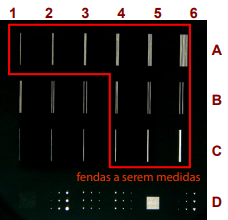
\includegraphics[scale=0.6]{figuras/rede_dif.png}
	\caption{Vidro e fendas utilizadas}
	\label{fig:rede}
\end{figure}

A fim de coletar os dados, buscando medir padrões de difração para fendas simples, o laser foi incidido na fenda C4, de forma que o padrão de difração pudesse ser observado em um papel milimetrado de $5x5\si{\milli\meter}$ utilizado como anteparo, posicionado a \SI{184,5}{\centi\meter}. O procedimento foi repetido para as fendas C5 e C6.

Para esta situação, o modelo de difração de Fraunhofer mostra que $\Delta y = 2\lambda z/b$, em que $\Delta y$ é a largura dos máximos, $z$ a separação entre o emissor de luz e o anteparo e $\lambda$ o comprimento de onda da luz emitida. Assim, dado que $z$ pode ser medidos experimentalmente, conhecendo o comprimento de onda é possível determinar a largura das fendas, sendo este o procedimento realizado pelo grupo.

Na sequência, foram medidos os padrões para fendas duplas e múltiplas. o mesmo procedimento anterior foi feito utilizando as fenda B4,B5 e B6 e A1 até A6, respectivamente. Vale ressaltar que para as fendas múltiplas, a abertura e separação era, nominalmente, a mesma.

Com fendas duplas o modelo de Fraunhofer mostra que a separação entre máximos (ou mínimos) de interferência é dada por $\Lambda = \lambda z/h$, onde $h$ é a separação entre as fendas. assim, de forma análoga ao processo para fendas simples, é possível determinar a separação entre as fendas a partir do comprimento de onda da luz emitida. Para determinação da largura das fendas, bastou aplicar o modelo de Fraunhofer para difração em fenda simples, já que para fendas duplas o fenômeno de difração também ocorre juntamente com interferência.

Ja para multíplas fendas, a largura dos máximos principais é dada por $\delta y = z\lambda/Nh$, em que N representa a quantidade de fendas. Utilizando esta equação, quando o número de fendas é grande e as mesma tem separação bem definida, é possível determinar o comprimento de onda da luz incidente.

A próxima etapa do experimento consistia da observação de padrões de difração com a luz incidindo em um fio de cabelo. foi utilizado um pequeno quadro de cartolina, de tamanho similar ao vidro utilizado anteriormente, com o fio de cabelo fixado em seu centro. A luz foi incidida no feixe e o padrão gerado foi observado no anteparo. Vale ressaltar que para essas condições, o modelo de Fraunhofer para fendas simples é aplicável, logo, para este padrão de difração,a determinação da largura do fio de cabelo é análoga a determinação da largura de uma fenda simples.

A última etapa de observações foi feita analisando os padrões de difração em aberturas variadas, em geral, não sendo fendas. O mesmo procedimento citado anteriormente foi realizado para as aberturas da coluna D, com intuito de inferir o tipo de abertura presente.

É importante ressaltar que em todos os procedimentos citados anteriormente fotos do anteparo foram tiradas a fim de analisar os padrões formados utilizando o \textit{software} \texttt{ImageJ}, determinando a distância entre mínimos de difração ($\Delta y$). Além disso, o grupo determinou que a resolução do papel e a medição do distanciamento do anteparo foram as principais fontes de incerteza a serem consideradas. Vale citar que outras fontes de incerteza, como o posicionamento (paralaxe) e resolução da câmera também foram identificadas porém não foram consideradas durante o processamento dos dados, pois se tratavam de incertezas de difícil abordagem e buscou-se minimiza-las durante o experimento.

Por fim, utilizando um microscópio metrológico, foram medidas as larguras das fendas ($b$), a separação entre as mesmas ($h$) e a quantidade de fendas ($N$) em para todas as situações anteriores. Evitou-se realizar medições repetidas nos caso em que as os valores medidos seriam iguais, como por exemplo de B4 a B6 em que a separação era idêntica e de A1 a A6, em que tanto a separação quanto a largura das fendas é igual. Para a utilização do microscópio metrológico, o grupo identificou a resolução do mesmo e paralaxe como incerteza.  


